\documentclass[a4paper]{article}

%% Language and font encodings
\usepackage[english]{babel}
\usepackage[utf8x]{inputenc}
\usepackage[T1]{fontenc}

%% Sets page size and margins
\usepackage[a4paper,top=3cm,bottom=2cm,left=3cm,right=3cm,marginparwidth=1.75cm]{geometry}

%% Useful packages
\usepackage{amsmath}
\usepackage{graphicx}

\usepackage[colorlinks=true, allcolors=blue]{hyperref}

\title{Plant-Id}
\author{Ethan Ahuja(ahujae) and Ethan Patterson(patteret)}

\begin{document}
\maketitle

\begin{abstract}
Plant-Id is a mobile application that implements a decision tree to identify different objects, such as plant species. This is accomplished by asking the user series of question, with each question asked the decision tree can narrow down a large list of species to a single organism.
\end{abstract}
\section{Introduction}
Plant-Id is a mobile application that can classifier different object. For example, but not limited to, classifying plant species. This application will be using a decision tree to identify what object a user is observing.
\section{Who is this for?}
If Plant-Id is trained to identify plant species. Those who would benefit from this application range from the casual to the professional. The curious hiker who is out in the middle of their hike comes across an intriguing plant and would like to know the name of this wonderful organism. A professional botanist might be in an a reign full of plant species that they are unfamiliar with and could use assistance with identifying the unknown organisms. 
\section{Limitations?}
Do to this being a student project plant species should be limited to the Corvallis area. This will help minimize some of the challenges in building this project. 
\section{Decision tree}
\subsection{What is it?}
\begin{figure}
\centering
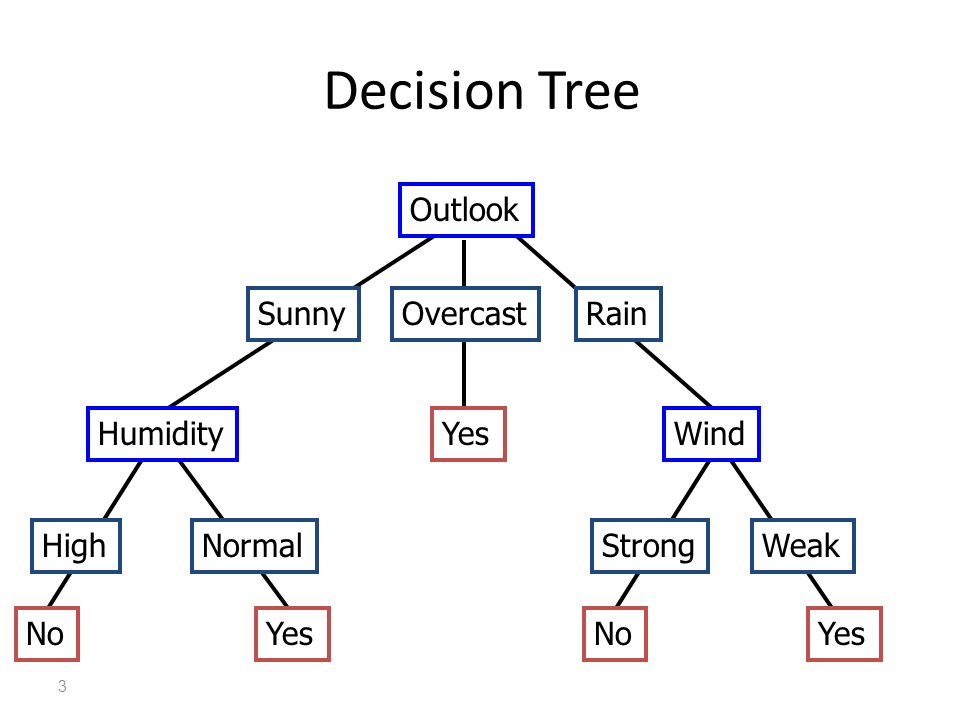
\includegraphics[width=0.4\textwidth]{Decision_Tree.jpg}
\caption{Sourse: http://www.saedsayad.com}
Should you go outside example
\end{figure}
A decision tree is a machine learning algorithm that asks a binary questions to reach a conclusion. It follows close to fundamental computer science notation of divide and conquer. Every question is binary allowing for the tree to sort through $2^N$ options, where N is the number of questions. For example 20 questions can sift through $2^{20}$ which is 1,048,576 options. Mapping these options creates a tree like structurer with the question being a parent node and the leafs being the yes or no response.
\begin{enumerate}
\centering
\item Should you go outside? as seen in figure 1.
\begin{itemize}
  \centering
  \item Program: Is it raining outside?
  \item User: Yes.
  \item Program: Is the wind strong?
  \item User: No.
  \item Program: You should go outside!
\end{itemize}
\end{enumerate}
\subsection{How it works}
A decision tree uses the an ID3 algorithm to build its tree like shape.ID3 uses entropy and information gain to build a tree.
\subsection{ID3 algorithm}
The ID3 algorithm is a top down greedy search. It builds a tee from a fixed training set. The resulting tree can then classify future samples.
\subsection{Entropy}
Data is partitioned into subsets that hold instances with homogeneous(similar) values. The ID3 algorithm uses entropy to calculate this homogeneous value. If the sample set is zero then the entropy is zero and if the set is equally divided, then the entropy is one. $$Entrepy frequency $$ $$E(S)\sum_{i=1}^{c} -p_{i} log_{2} p_{i}$$ $$Source: www.saedsayad.com$$
\subsection{Information gain}
Information gain is the decrease in entropy after a dataset is split on an attribute. One will want to find the highest homogeneous branches.
\section{Resources}
The decision tree will require a training and a test data sample to train on. This will require team members to gather information bout plants in the Corvallis area to build these data sets to train from, the more data collected the more accurate one can train the tree to be. Information on how to identify a plant can be found from the library on campus or through Google searches.
\section{Challenges}
The most challenging part of this task for students will be how to gathering data and then organizing this data in a useful way for the ID3 algorithm to sift through. A big goal will be to figure out what questions to ask and in what order to ask them.
\section{Previous approaches.}
The application Garden Answers Plant ID by TeamSOA, Inc, as seen in the app store is a plant identifier that uses a neural network to identify photos of plants, and give users useful information about the scanned plant. Plant Classifier will instead use a decision tree to identify the plant. This will allow the developers of Plant Classifier to add new species at a faster rate and help inform users what features they should be looking for on a plant to successfully identify the species.
\section{Hardware Software recommendations}
The recommended hardware is a phone running an android operating system. A developers machine should have 8 GB RAM 500 MB disk storage and Java (JDK) 8 to run the Android studio's IDE.
\newpage %Move references to the next page..
\begin{thebibliography}{9}
\bibitem{latexcompanion} 
\url{http://www.saedsayad.com/decision_tree.htm}
Dr. Saed Sayad, Reading, www, 2010-2018.
\bibitem{einstein} 
Victor Lavrenko.
\url{https://www.youtube.com/watch?v=eKD5gxPPeY0&list=PLBv09BD7ez_4temBw7vLA19p3tdQH6FYO}
\textit{School of Informatics} 
[\textit{Decision Trees}]. 
Victor Lavrenko and Nigel Goddard, January 19, 2014.
\end{thebibliography}
\end{document}